\chapter{\MakeUppercase{Estado del Arte}} \label{Estado del Arte}
\thispagestyle{mainmatterstyle} % Cambia el estilo para que este numerado en la esquina superior derecha. Esta presente en todos los chapter

En este capítulo se presenta una revisión de trabajos de investigación, sistemas comerciales y patentes relacionados al control de calidad automático de prendas de vestir.

\section{Investigaciones Académicas}

\subsection{System of error detection in the manufacture of garments using artificial vision}

El sistema desarrollado la investigación \cite{Moreno2017} consiste en un sistema de visión artificial implementado para detectar errores en la etapa de corte durante el proceso de fabricación de prendas en la industria textil. Utiliza un sistema embebido Raspberry Pi 3, equipado con el sistema operativo basado en Linux Raspbian y el compilador OpenCV para el desarrollo de códigos de visión por computadora. Este sistema, que se muestra en \ref{fig:luz_sistema}, logra segmentar perfectamente las prendas independientemente del color que se les haya dado en procesos anteriores, gracias a la implementación de un fondo dinámico opaco compuesto por LEDs RGB que cambian de color dependiendo del contraste con la prenda.

\begin{figure}[H]
	\centering
	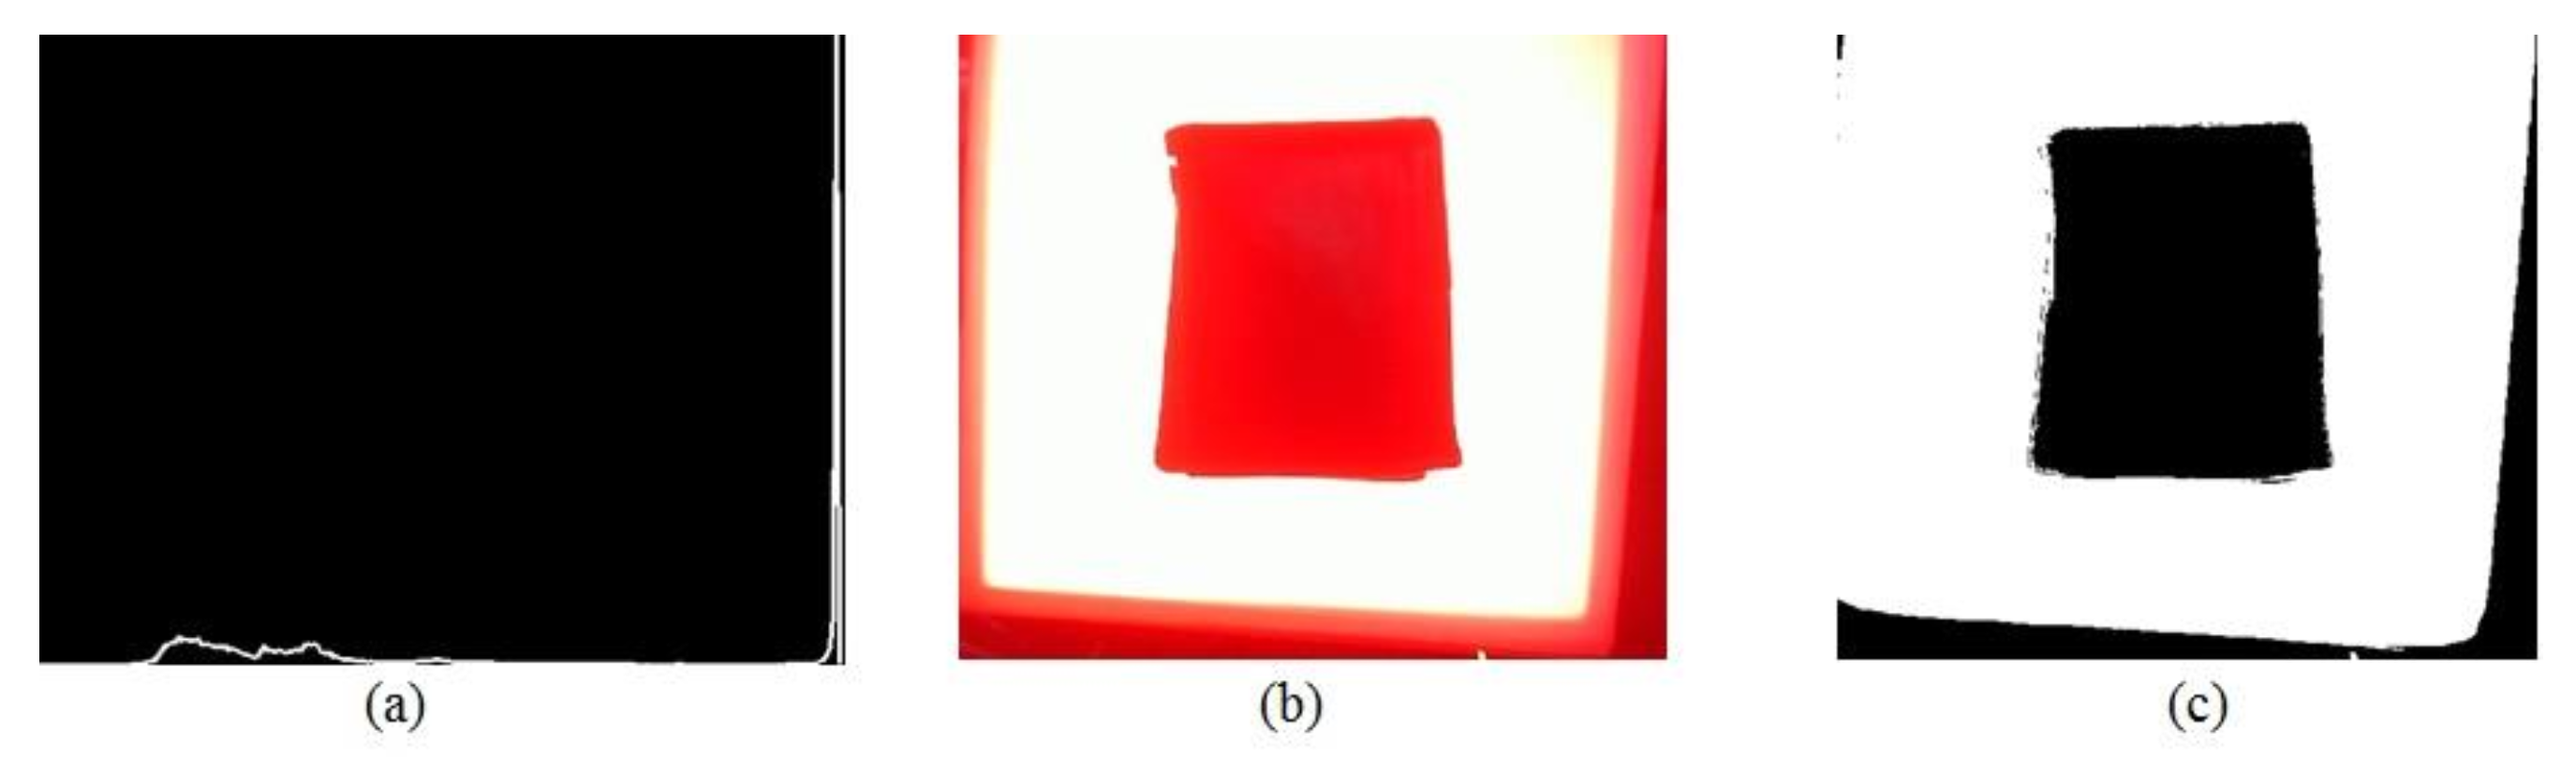
\includegraphics[width=0.8\textwidth]{img/luz_sistema.png}
	\caption[Sistema de visión artificial con fondo dinámico.]{Sistema de visión artificial con fondo dinámico. Fuente \cite{Moreno2017}.}
	\label{fig:luz_sistema}
\end{figure}

El algoritmo principal del sistema inicia con la captura de la imagen de la prenda, seguido por el promedio de cada canal de la imagen completa (rojo, verde y azul). Luego, se cambia el color del fondo basándose en el color que menos presencia tenga en la imagen, utilizando combinaciones de colores primarios en los LEDs RGB para minimizar el consumo de corriente. Finalmente, se captura una nueva imagen con el fondo bien contrastado con la prenda para verificar el contraste correcto.

\subsection{Using object detection technology to identify defects in clothing for blind people}

En la investigación \cite{Rocha2023} se muestra como la tecnología de detección de objetos, específicamente la arquitectura You Only Look Once (YOLO), ha sido aplicada de manera innovadora para ayudar a las personas ciegas a identificar defectos, como manchas o agujeros, en su ropa. Este enfoque utiliza un sistema de detección de defectos basado en el aprendizaje profundo para categorizar y detectar estas imperfecciones en prendas de vestir, lo que representa un paso importante hacia la mejora de la autonomía y la confianza de las personas ciegas en la selección de su vestimenta. El sistema propuesto en este estudio se basa en la recolección de un conjunto de datos específico de ropa con defectos, el cual es utilizado para entrenar y evaluar el sistema. La metodología empleada para optimizar el sistema de detección de defectos incluye aumentar el conjunto de datos con nuevos defectos, condiciones de iluminación y fondos, introducir la ampliación de datos y la clasificación de defectos, demostrando ser eficaz y adecuado para diferentes condiciones de detección de defectos desafiantes.

\begin{figure}[H]
	\centering
	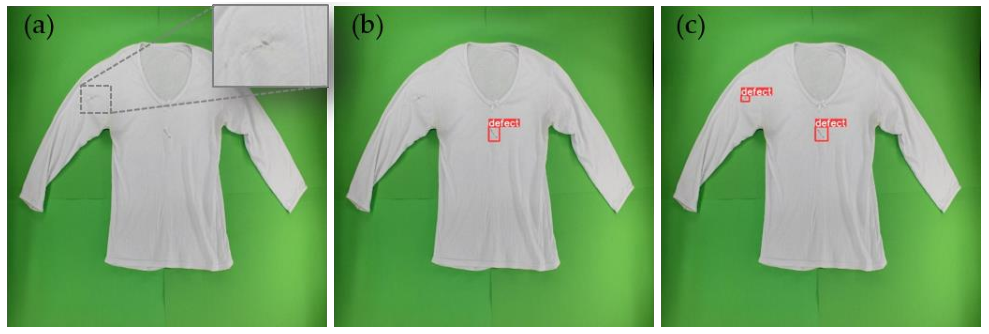
\includegraphics[width=0.9\textwidth]{img/example_YOLO.pdf}
	\caption[Defecto ignorado por YOLOv5m6, detectado tras la ampliación de datos.]{Defecto ignorado por YOLOv5m6, detectado tras la ampliación de datos desarrollada por \cite{Rocha2023}: (a) imagen original, (b) imagen predicha por el modelo YOLOv5m6 sin ampliación, y (c) imagen predicha por el modelo YOLOv5m6 con ampliación.}
	\label{fig:example_YOLO}
\end{figure}

El trabajo futuro en este campo se centra en la creación de una aplicación móvil y un sistema mecatrónico, como un armario automático, que incorpore los algoritmos y metodologías desarrolladas. Esto no solo pone de manifiesto la utilidad práctica de la tecnología de detección de objetos para la comunidad ciega, sino que también abre la puerta a aplicaciones automáticas que pueden facilitar aún más la gestión del vestuario por parte de las personas con discapacidad visual, proporcionando una herramienta de apoyo esencial para su independencia y confianza en la vida cotidiana. Este enfoque innovador destaca el potencial de las tecnologías de visión por computadora en la asistencia y mejora de la calidad de vida de las personas con discapacidades visuales.

\subsection{Automatic Measurement of Garment Sizes Using Image Recognition}

El documento presenta una innovadora metodología para medir automáticamente las tallas de prendas de vestir utilizando tecnología de reconocimiento de imágenes mediante el dispositivo que se muestra en la Figura \ref{fig:Automatic_Measurement}. Al enfrentar el problema de altas tasas de devolución en la moda en línea, debido a las inconsistencias en las tallas entre diferentes marcas y fabricantes, este estudio propone una solución tecnológica que combina el diseño de un conjunto de equipos especializados para capturar imágenes de prendas extendidas y un enfoque de medición automática basado en plantillas de prendas. Estas plantillas permiten identificar el tipo de prenda y puntos de características clave para calcular sus tallas. Este método ofrece una herramienta útil y eficiente para la medición de prendas, mostrando resultados precisos que satisfacen los requisitos de la industria del vestido, y tiene el potencial de mejorar significativamente la experiencia de compra en línea al reducir la tasa de devoluciones gracias a una estandarización en la medición de tallas \cite{Li2017AutomaticMeasurement}.

\begin{figure}[h]
	\centering
	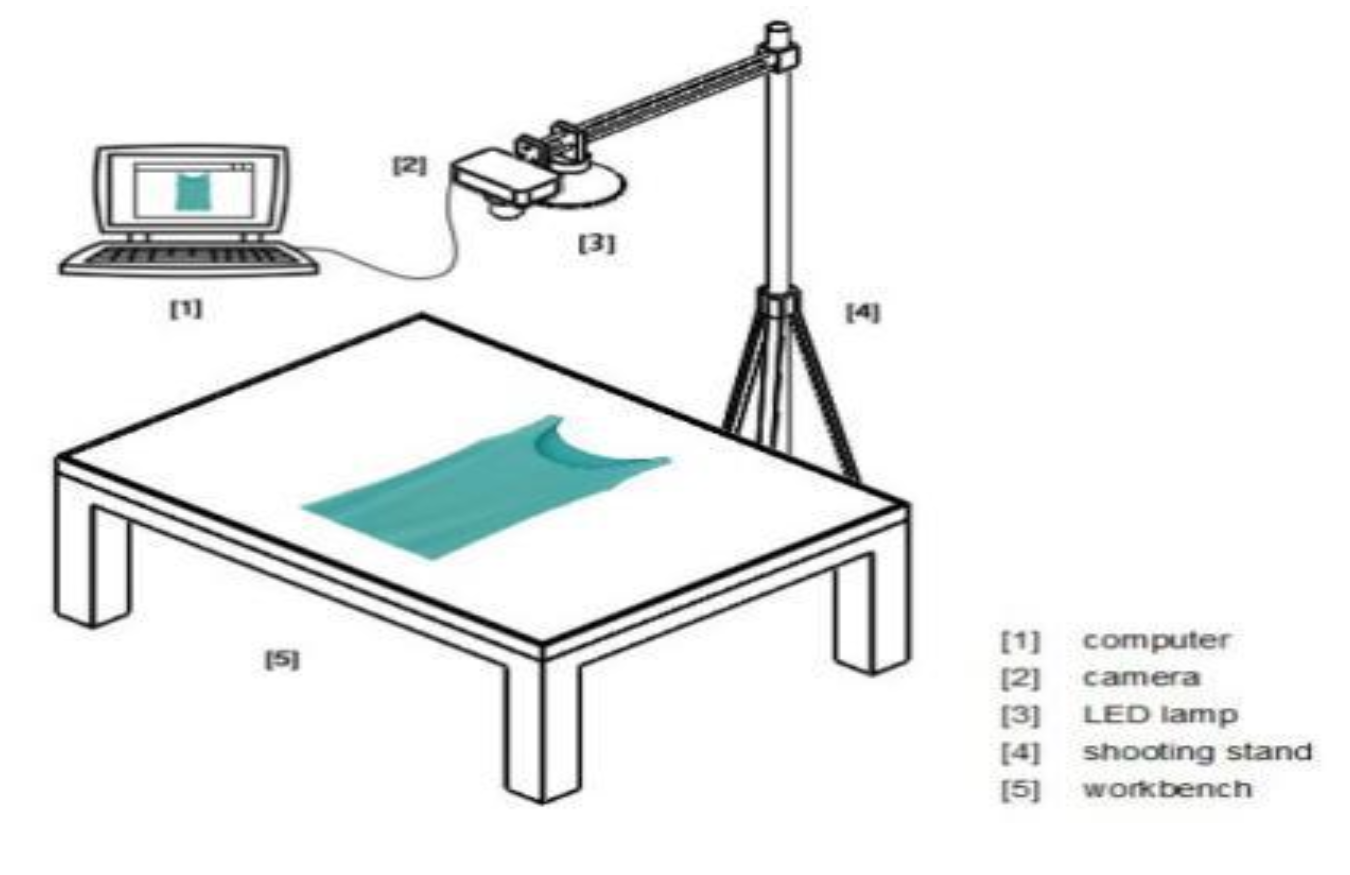
\includegraphics[width=0.6\textwidth]{img/Automatic_Measurement.png}
	\caption[Diseño de un dispositivo para medición automática de tallas de prendas mediante reconocimiento de imágenes]{Diseño de un dispositivo para medición automática de tallas de prendas mediante reconocimiento de imágenes. Fuente \cite{Li2017AutomaticMeasurement}.}
	\label{fig:Automatic_Measurement}
\end{figure}

\section{Productos Comerciales}

\subsection{Handheld Needle Detector ON-30}

En el contexto de la detección de metales en la industria textil, el Detector de Agujas Portátil ON-30 de Oshima, que se muestra en la Figura \ref{fig:oshima_on_30} se presenta como una herramienta eficaz. Este dispositivo, alimentado por baterías AA y basado en inducción magnética, se destaca por su capacidad para identificar con precisión objetos metálicos pequeños. Su diseño compacto y la implementación de alarmas visuales y sonoras facilitan su uso en diversas situaciones, ofreciendo una solución práctica para garantizar la seguridad en los procesos de producción textil \cite{oshimaEfficientHandheld}. Las características de este producto se observan en el Cuadro \ref{tab:specs_ON_30}.

\begin{figure}[H]
	\centering
	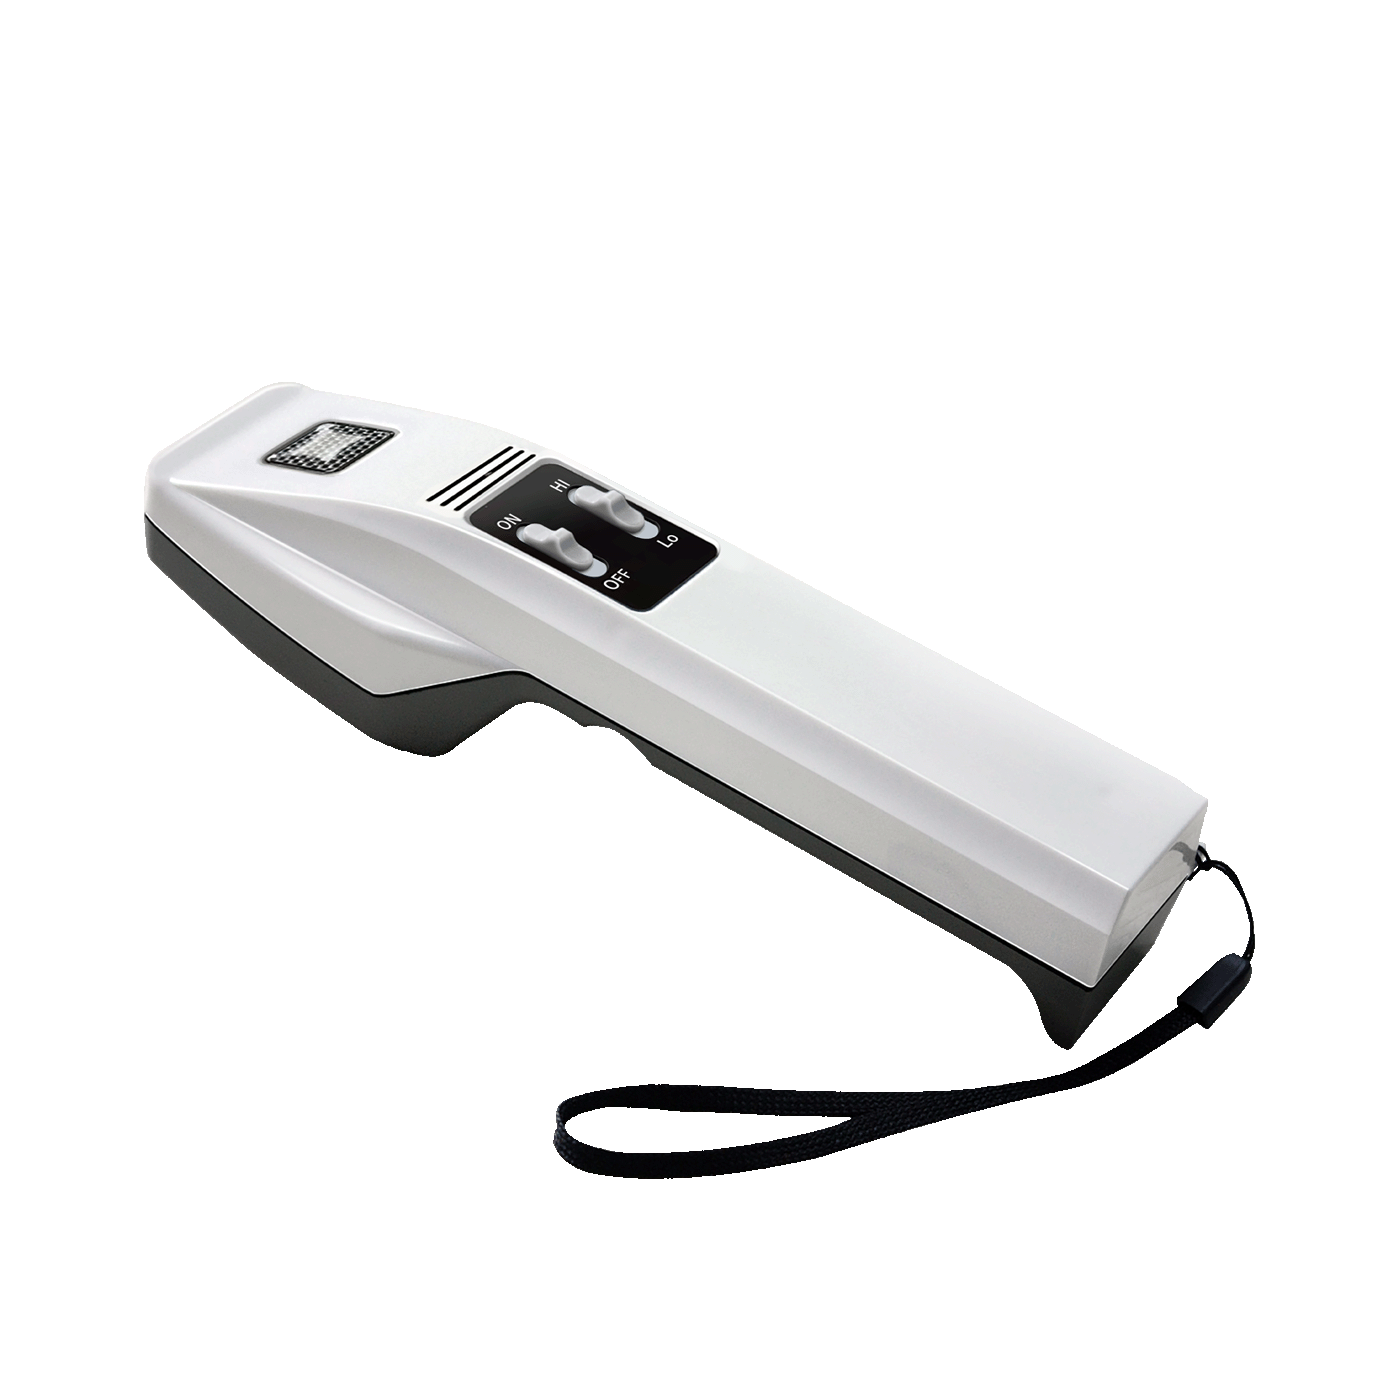
\includegraphics[width=0.4\textwidth]{img/oshima_on_30.png}
	\caption{Detector de Agujas Portátil ON-30 de Oshima.}
	\label{fig:oshima_on_30}
\end{figure}

\begin{table}[H]
	\caption{Especificaciones del Modelo ON-30.}
	\begin{tabularx}{\textwidth}{|l|X|}
		\hline
		\textbf{Característica} & \textbf{Especificación} \\ \hline
		Modelo & ON-30 \\ \hline
		Fuente de Alimentación & Batería 6F22-9V, corriente de reposo del LED <5mA. Alarma de sonido y luz. Corriente dinámica <30mA, corriente dinámica de la alarma de vibración <60mA, ahorro de energía. \\ \hline
		Sensibilidad & La inspección cercana puede detectar una bola de hierro de 0.5 mm, una bola de hierro de 1.2 mm de diámetro hasta una altura de 10 mm. La máxima sensibilidad puede detectar una bola de hierro de 0.8 mm de diámetro, un pasador de ruptura de 0.7 x 20 de diámetro hasta una altura de 50 mm. \\ \hline
		Método de Detección & Inducción magnética \\ \hline
		Espacio de Detección (mm) & 70x55 \\ \hline
		Alarma & Zumbador, lámpara \\ \hline
		Dimensiones LxAxA (mm) & 195x58x50 \\ \hline
		Volumen del Empaque LxAxA (mm) & 250x100x55 \\ \hline
		Peso Neto/Peso Bruto (kg) & 0.212/0.35 \\ \hline
	\end{tabularx}
	\label{tab:specs_ON_30}
\end{table}

\subsection{Digital Conveyor Needle Detectors ON-688CD6S/688CDD6S}

Los detectores de agujas para cinta transportadora ON-688CD6S/688CDD6S de OSHIMA incorporan sensores de 10 puntos para una mayor sensibilidad y confiabilidad, con ajuste de sensibilidad en tres niveles para diferentes necesidades de detección. Su interfaz de pantalla táctil facilita su uso, y la máquina es capaz de conectarse a datos, contabilizar productos, y calibrarse automáticamente cada dos horas \cite{oshimaOSHIMAGarment}. Las especificaciones de estos modelos se muestran en la Tabla \ref{tab:specs_ON-688CD6S/688CDD6S}.

\begin{figure}[h]
	\centering
	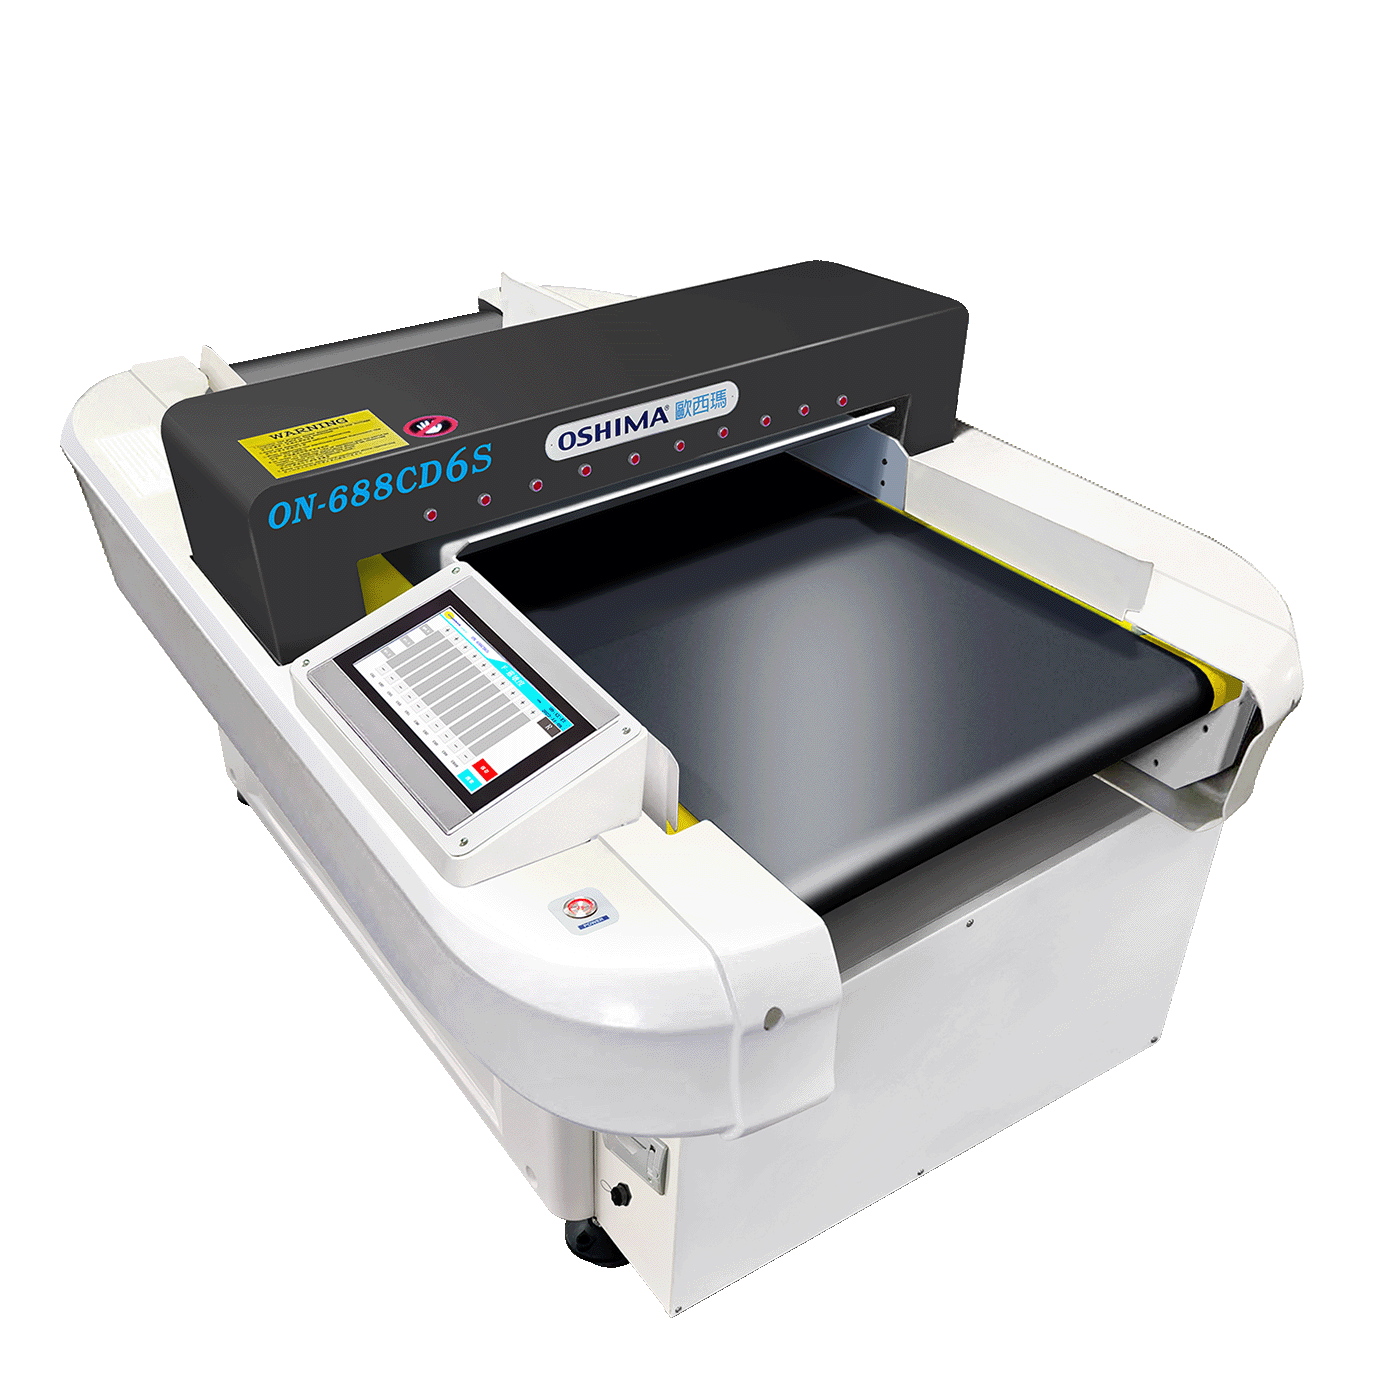
\includegraphics[width=0.5\textwidth]{img/oshima_conveyor.png}
	\caption{Detectores de agujas para cinta transportadora ON-688CD6S/688CDD6S.}
	\label{fig:oshima_conveyor}
\end{figure}

\begin{table}[H]
	\caption{Especificaciones de los modelos ON-688CD6S/688CDD6S.}
	\begin{tabularx}{\textwidth}{|X|X|X|}
		\hline
		\multirow{2}{*}[2pt]{\textbf{Característica}} & \multicolumn{2}{c|}{\textbf{Especificaciones}} \\ \cline{2-3}
		& \textbf{ON-688CD6S} & \textbf{ON-688CDD6S} \\
		\hline
		Detecting tower & Single tower & Double tower \\
		\hline
		Detective height (mm) & 100 & 100 \\
		\hline
		Detective width (mm) & 600 & 600 \\
		\hline
		Effective detecting Height (mm) & 90 & 90 \\
		\hline
		Power supply & 1P AC220V 50/60Hz & 1P AC220V 50/60Hz \\
		\hline
		Rate (kW) & 0.2 & 0.2 \\
		\hline
		Detective capability of iron ball (mm) & Fe 0.8/1.0/1.2 & Fe 0.8/1.0/1.2 \\
		\hline
		Sensitivity adjustment & Level adjustment & Level adjustment \\
		\hline
		Conveyor speed (m/min) & 32 & 32 \\
		\hline
		Detection method & Magnet & Magnet \\
		\hline
		Alarm & Automatic buzzer and alarm indicator light, the conveyor rewinding function & Automatic buzzer and alarm indicator light, the conveyor rewinding function \\
		\hline
		Dimensions LxWxH (mm) & 1720X1100X920 & 1820X1180X1100 \\
		\hline
		Packaging volume LxWxH (mm) & 2160X1060X920 & 2330X1130X1100 \\
		\hline
		N.W/G.W (kg) & 280/380 & 420/570 \\
		\hline
	\end{tabularx}
	\label{tab:specs_ON-688CD6S/688CDD6S}
\end{table}

\subsection{AI-Driven Measurement Checking Machine}

Este desarrollo tecnológico, el cual se muestra en la Figura \ref{fig:inspection_machine} de la empresa Dongguan Yunji Zhihui Technology facilita la automatización de procesos previamente manuales, por lo que augura reducciones significativas en los costos laborales y mejoras en el control de calidad \cite{RMG2021AIGarment}. Las especificaciones de este sistema se muestran en la Tabla \ref{tab:spec_inspection_machine}.

\begin{figure}[H]
	\centering
	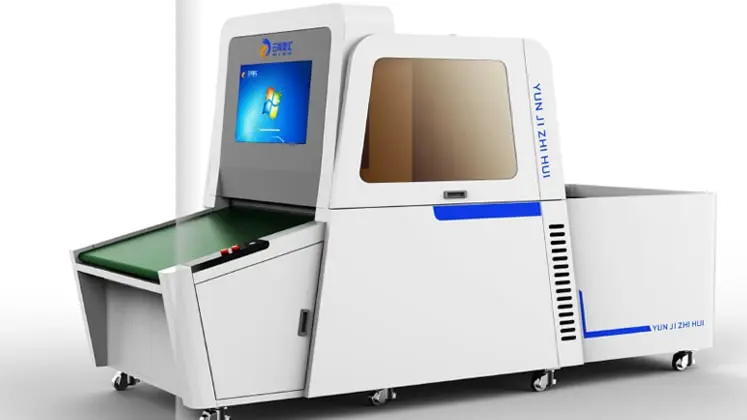
\includegraphics[width=0.7\textwidth]{img/inspection_machine.png}
	\caption[Máquina de chequeo de medidas conducido por IA.]{Máquina de chequeo de medidas conducido por IA. Fuente \cite{RMG2021AIGarment}.}
	\label{fig:inspection_machine}
\end{figure}

\begin{table}[H]
	\centering
	\caption[Características cuantitativas del sistema de inspección de prendas con IA.]{Características cuantitativas del sistema de inspección de prendas con IA. Fuente: Elaboración propia.}
	\begin{tabular}{|l|l|}
		\hline
		\textbf{Característica} & \textbf{Valor} \\ \hline
		Dimensiones medidas por prenda & 15 dimensiones \\ \hline
		Tiempo por artículo & Máximo 6 segundos \\ \hline
		Capacidad de procesamiento & 4800 camisetas en 480 minutos \\ \hline
		Precisión de medición & Error dentro de ±1 mm \\ \hline
		Exactitud de detección & Hasta el 99.5\% \\ \hline
		Adaptabilidad & Ajuste según color y tela de las prendas \\ \hline
	\end{tabular}
	\label{tab:spec_inspection_machine}
\end{table}

\section{Patentes}

\subsection{US20200178632A1}
La invención \cite{us20200178632a1} describe un aparato, método y sistema de control automatizado para mejorar la inspección, medición y fabricación de prendas de vestir como se observa en la Figura \ref{fig:US20200178632A1-20200611-D00005}. Este sistema captura una imagen de la prenda la convierte en una representación digital que puede enviarse y almacenarse en una base de datos. Esta información digital se utiliza para recrear prendas ideales con medidas y patrones reproducibles. Además, el sistema permite comparaciones con imágenes ideales existentes y/o con la propia prenda para determinar si posee las dimensiones, formas, colores, texturas y tejidos correctos.

\begin{figure}[H]
	\centering
	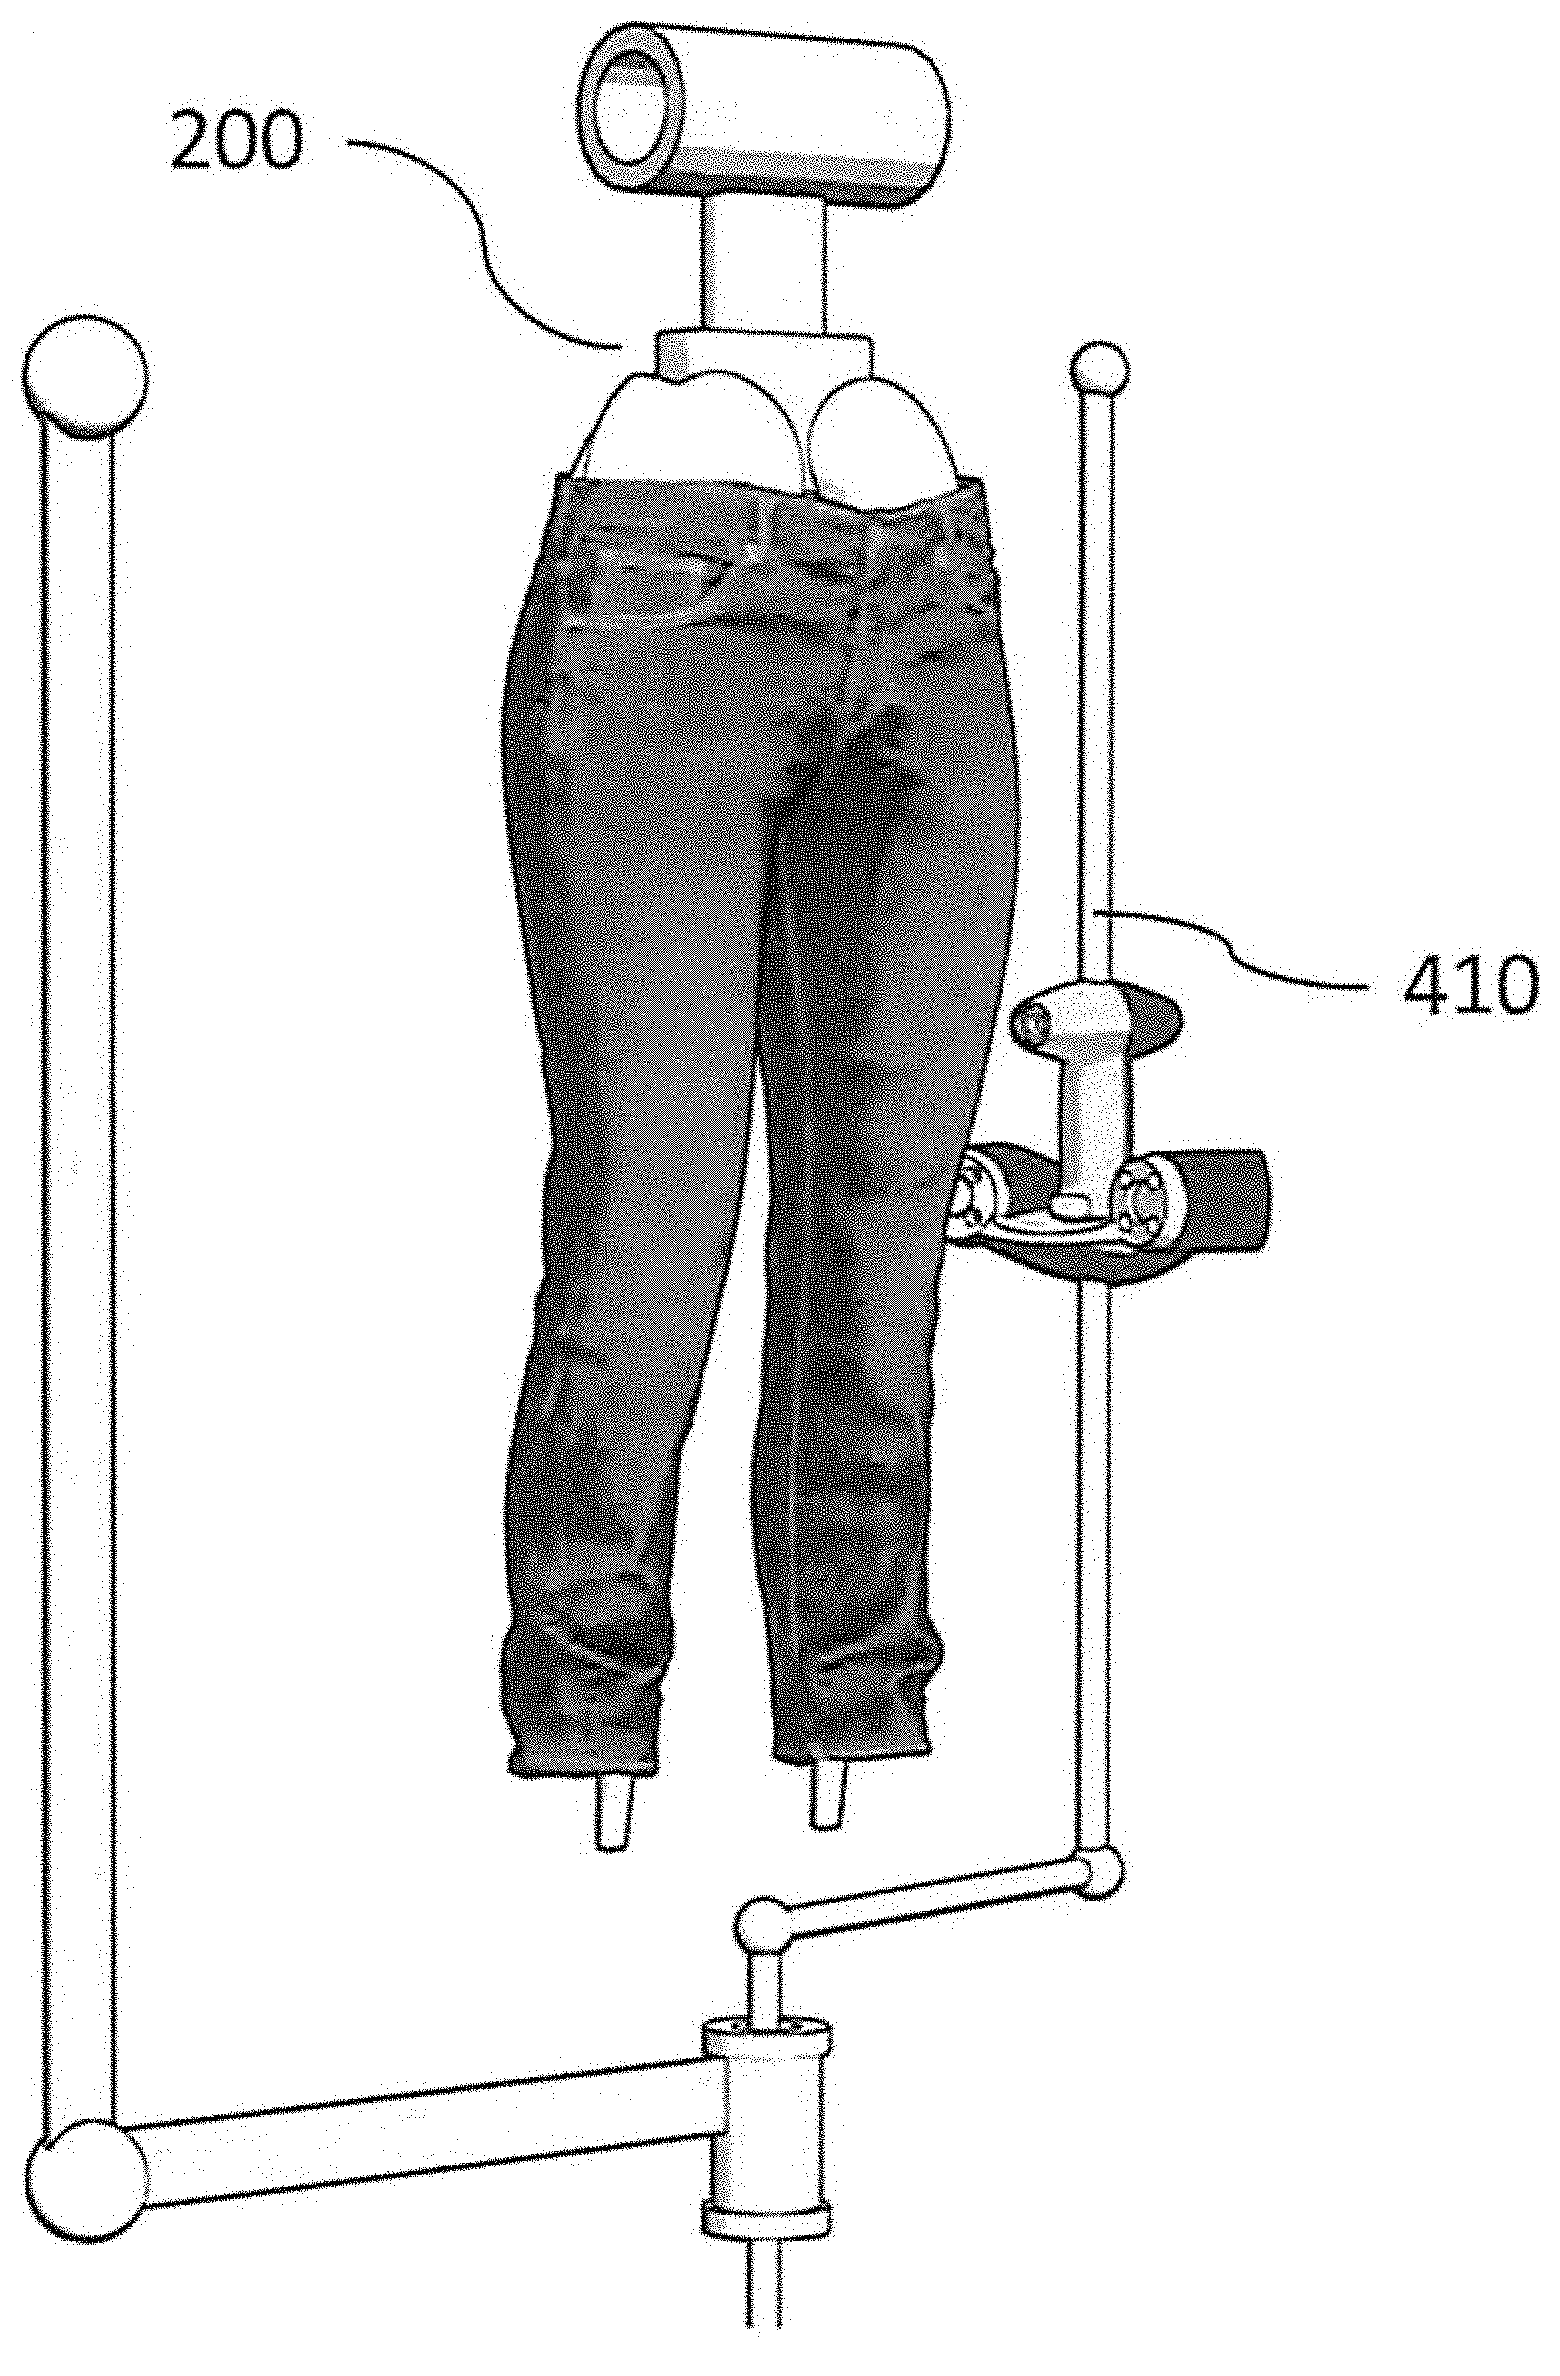
\includegraphics[width=0.3\textwidth]{img/US20200178632A1-20200611-D00005.png}
	\caption{Patente con captura de detalles en 3D.}
	\label{fig:US20200178632A1-20200611-D00005}
\end{figure}

\subsection{US5530652A}

La invención \cite{US5530652A} detalla un sistema que incluye técnicas de escaneo 3D (ópticas o electroópticas) para adquirir datos de escaneo dimensionales. Estos datos se procesan para la extracción de medidas y retroalimentación. La organización de los datos permite su almacenamiento y recuperación, finalizando con el control de medidas de las prendas, la fabricación y la categorización basada en la retroalimentación.

Este sistema se destaca por su capacidad para automatizar el control y la inspección de la calidad de las prendas producidas, minimizando la necesidad de contacto humano directo con los objetos, lo que facilita un análisis dimensional preciso y automatizado. La tecnología descrita en esta patente tiene potencial para revolucionar la forma en que se miden, inspeccionan y fabrican las prendas de vestir, asegurando consistencia y calidad en la producción de vestimenta.

La patente US5530652 describe un sistema automático de inspección y medición de prendas que puede crear representaciones electrónicas bidimensionales o tridimensionales de un objeto. Estas representaciones pueden ser combinadas con otras para crear una base de datos de medidas de donde se pueden generar patrones estándar para su uso en la fabricación de prendas. Además, la representación electrónica puede utilizarse para comparar el objeto fabricado con una representación ideal, determinando si las medidas del objeto se encuentran dentro de una tolerancia predeterminada respecto a la representación ideal. Se emplea un sistema de visión por máquina para capturar una imagen del objeto y convertirla en una representación digital, que luego puede agregarse a una base de datos para compilar un patrón ideal o compararse con una imagen ideal existente para verificar si el objeto tiene el tamaño correcto.

La patente aborda el desarrollo de un método y un sistema para la inspección y medición automática de prendas, con el objetivo de asegurar que las dimensiones de las prendas fabricadas se ajusten a los estándares ideales y tolerancias predefinidas. Esto facilita la creación de bases de datos de medidas que pueden utilizarse para mejorar la fabricación de prendas, asegurando una mayor precisión y consistencia en el tamaño y la calidad de las prendas producidas.

\begin{figure}[H]
	\centering
	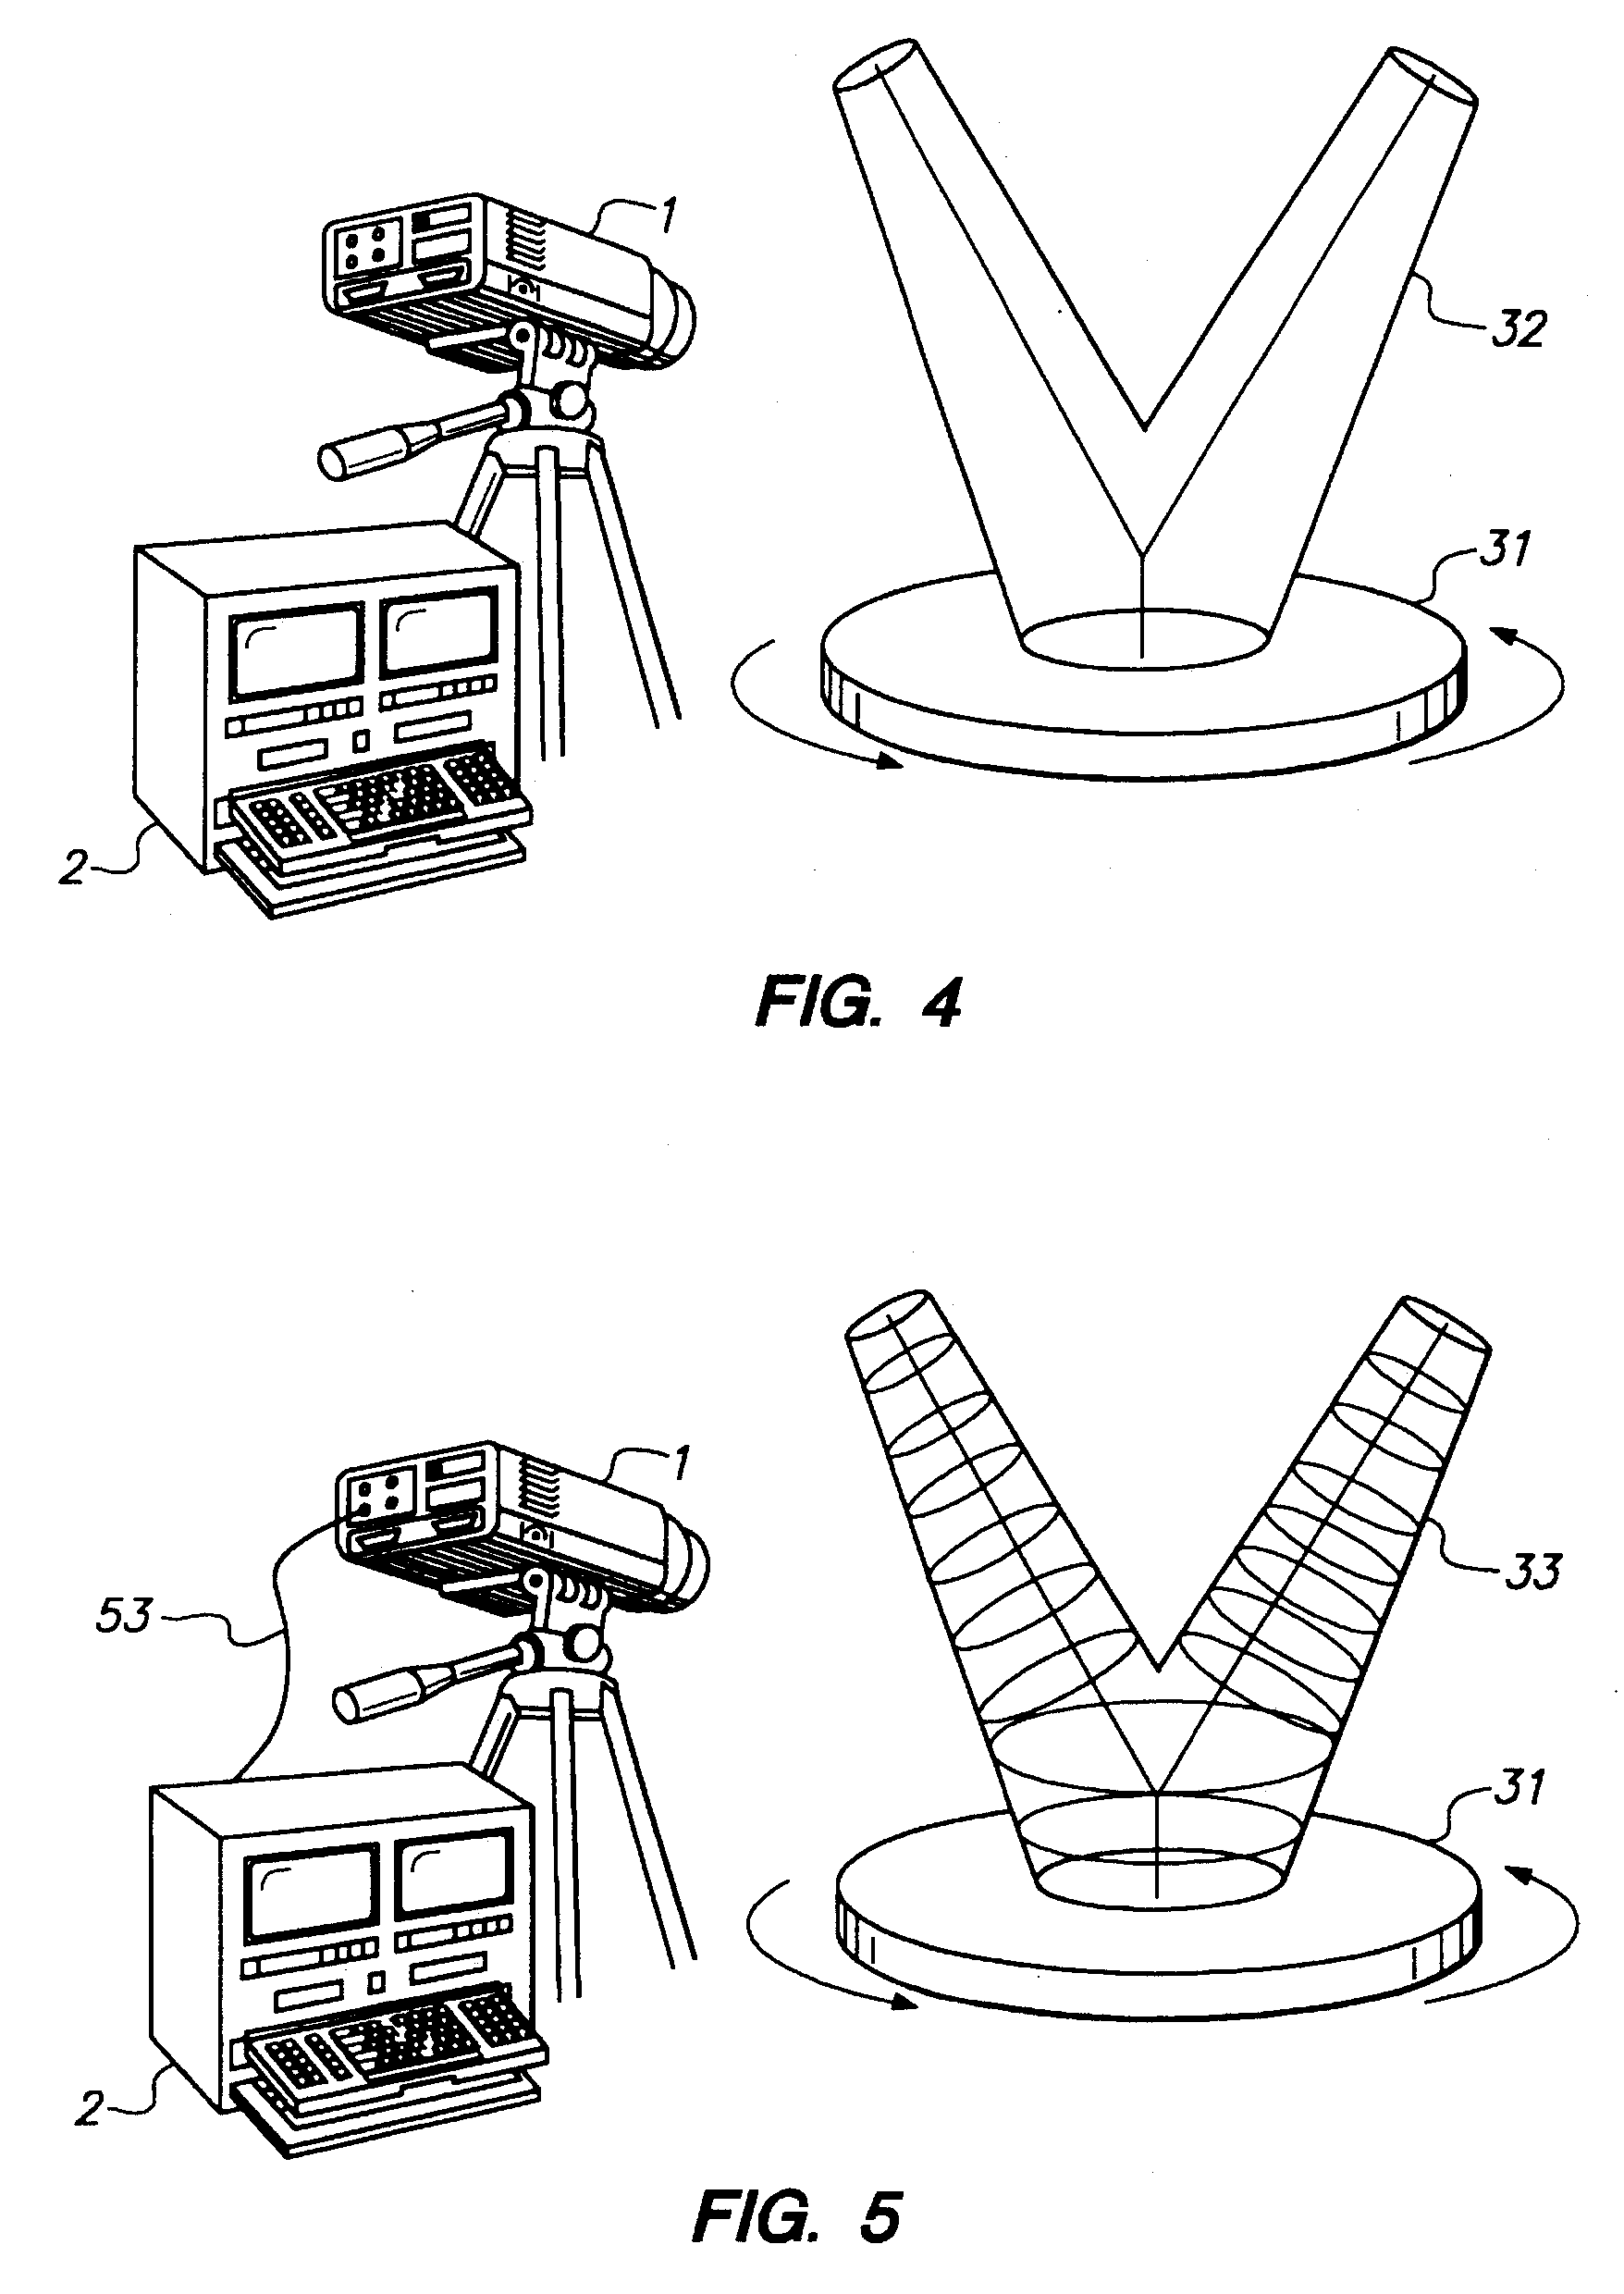
\includegraphics[width=0.3\textwidth]{img/US5530652-drawings-page-7.png}
	\caption[Sistema de captura y digitalización.]{Sistema de captura y digitalización. Fuente \cite{US5530652A}.}
	\label{fig:US5530652-7}
\end{figure}

\begin{figure}[H]
	\centering
	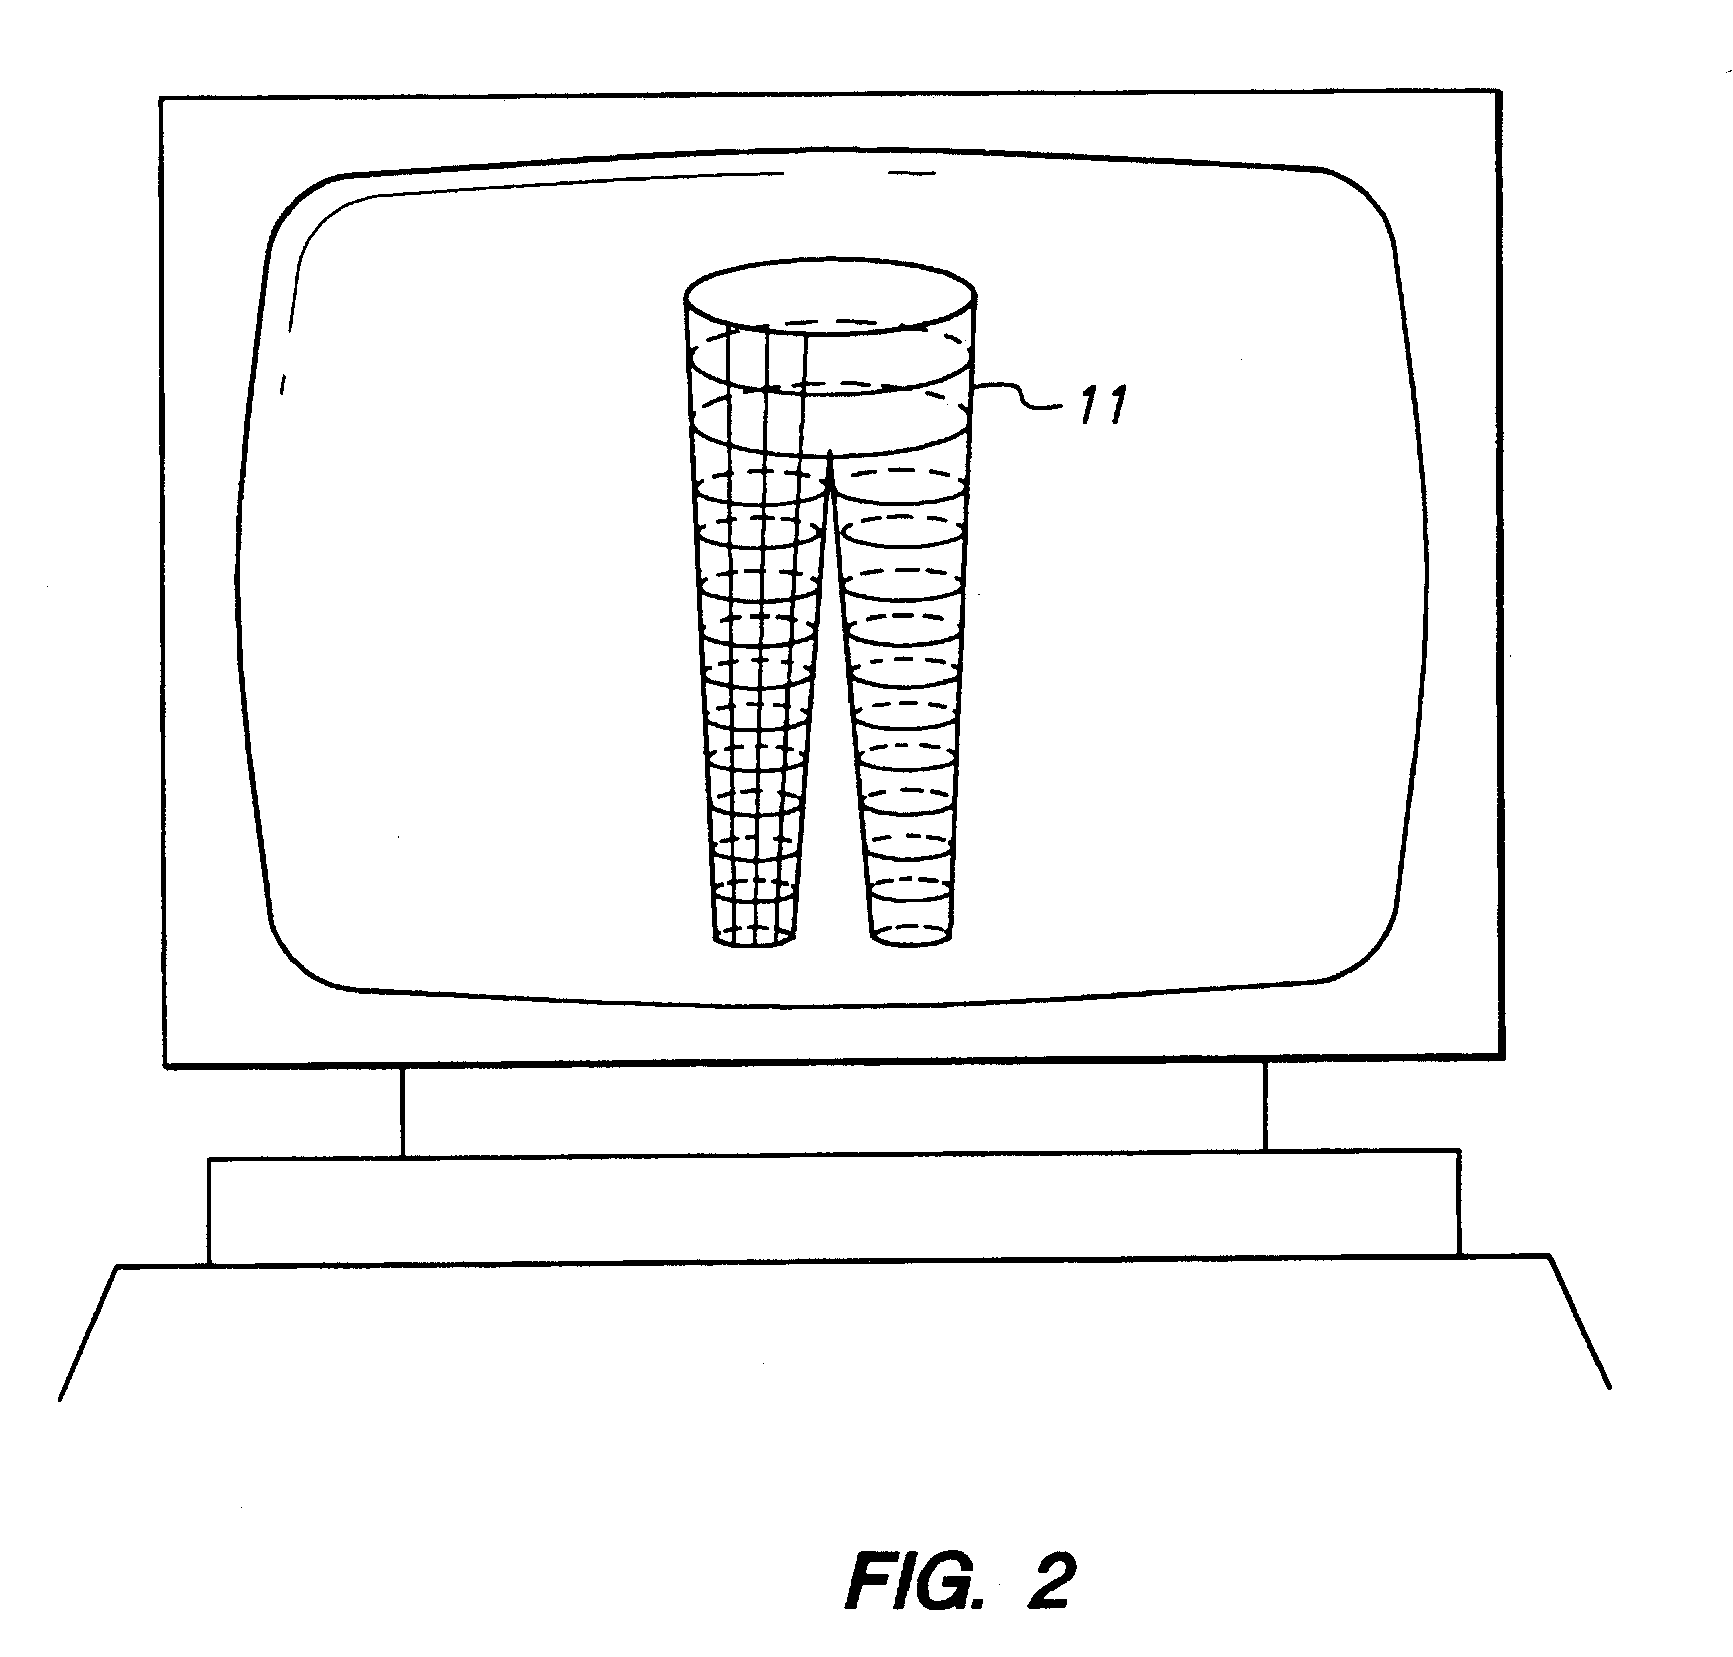
\includegraphics[width=0.4\textwidth]{img/US5530652-drawings-page-5.png}
	\caption[Digitalización de la prenda.]{Digitalización de la prenda. Fuente \cite{US5530652A}.}
	\label{fig:US5530652-5}
\end{figure}

\subsection{EP4095520A1}

La patente \cite{EP4095520A1} describe un sistema para el control de calidad de prendas de vestir, diseñado para identificar de manera automática y objetiva defectos tanto visibles como invisibles en la estructura interna de las prendas. Este sistema, como se observa en la Figura \ref{fig:imgf0001} se compone de dos elementos principales: un mecanismo para insuflar un gas de control a una temperatura al menos 20°C superior a la temperatura ambiente en la prenda, y un medio de captura de imágenes para detectar ubicaciones defectuosas en dicha prenda. El gas de control calentado, como aire caliente o vapor, permite detectar defectos gracias a la diferencia de temperatura que se genera en las zonas dañadas o perforadas, sin causar daño adicional a la prenda durante la inspección.

El sistema también puede incluir cámaras térmicas o de luz visible, medios para visualizar el vapor que pasa a través de la prenda y software para generar una imagen 3D de la prenda que facilita la identificación y localización precisa de los defectos. Este enfoque permite un alto grado de automatización y precisión en la detección de defectos, ofreciendo la posibilidad de determinar la naturaleza y severidad de los defectos detectados para posibles reparaciones. Además, el sistema puede ser utilizado para controlar la calidad de prendas de vestir técnicas o de alto rendimiento, asegurando que cumplan con los estándares de calidad requeridos a lo largo de su ciclo de vida, incluso después de múltiples usos y lavados.

\begin{figure}[H]
	\centering
	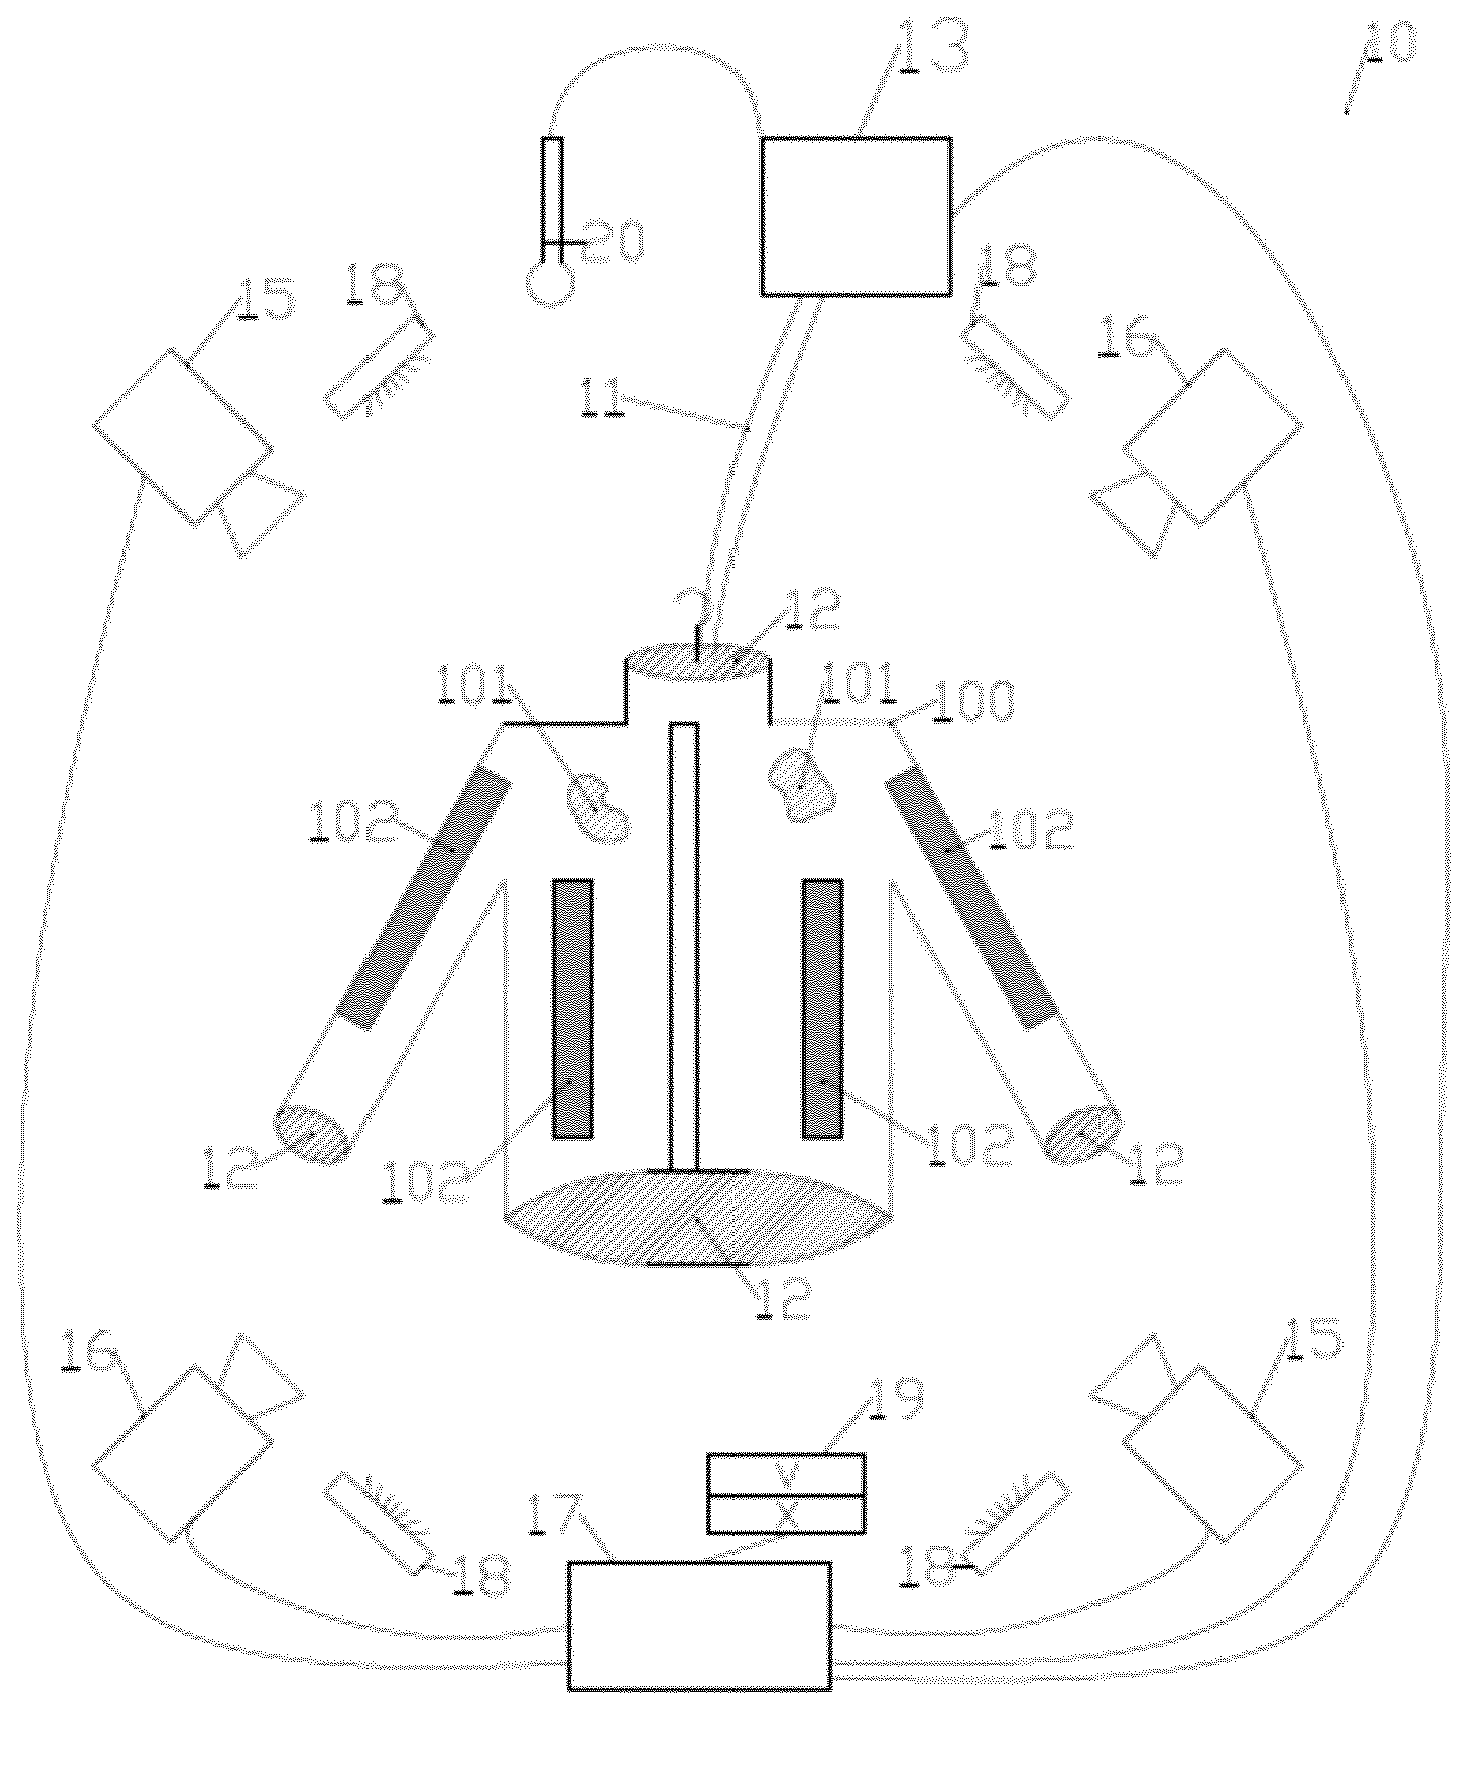
\includegraphics[width=0.4\textwidth]{img/imgf0001.png}
	\caption{Sistema de control de calidad con un mecanismo para insuflar gas.}
	\label{fig:imgf0001}
\end{figure}
